\documentclass[spanish,12pt,letterpapper]{article}
\usepackage[utf8]{inputenc}
\usepackage{graphicx}
\begin{document}
	\begin{titlepage}
		\begin{center}
			
\includegraphics[width=0.6\textwidth]{./logoUnADM}~\\[1cm] 
			\textsc{Universidad Abierta y a Distancia de México}\\[0.8cm]
			\textsc{Desarrollo de Software}\\[1.8cm]
			
			\textbf{ \Large Actividad 2. Metodología UML}\\[3cm]
			
			Diego Antonio Plascencia Lara\\ ES1421004131 \\[0.4cm]
			Facilitador(a): Julia Alicia Reyes Rios\\
			Materia: Modelado de Negocios\\
			Grupo: DS-DMDN-1601-B1-007 \\
			Unidad: I \\
			
			\vfill México D.F\\{\today}
			
		\end{center}
	\end{titlepage}
	
	\section{Introducción\\}
	Para esta actividad he elegido el proceso principal de una Startup: el desarrollo de cliente, que se puede dividir en Búsqueda y Ejecución, a su vez estas se subdividen en 4 actividades que son las que represente en el diagrama con ayuda de artefactos UML. Decidí hacer el diagrama en ingles para conservar los conceptos del proceso descrito en Lean Startup.\\
	
	\begin{center}
	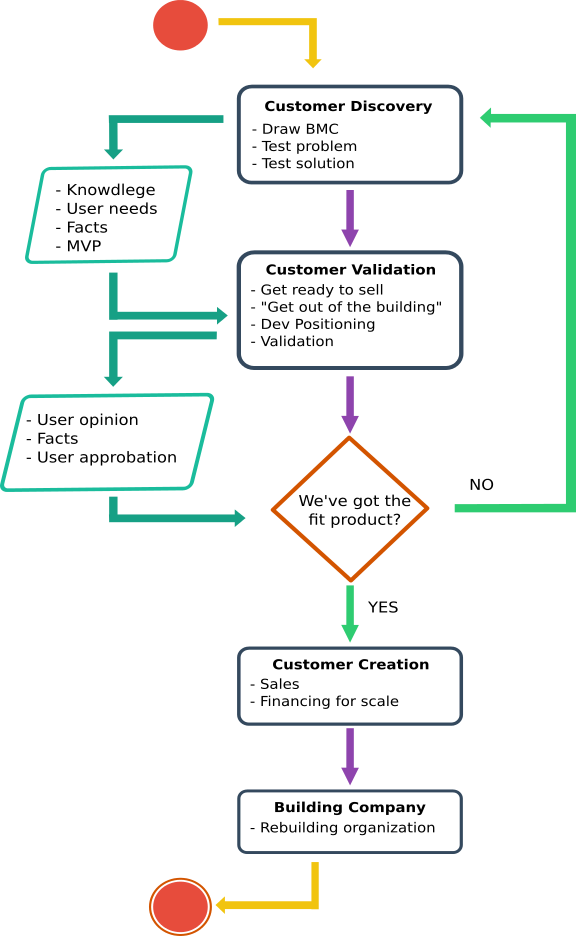
\includegraphics[width=0.6\textwidth]{./diagram}~\\[0.5cm]
	\end{center}
	
	
	\pagebreak
	\begin{thebibliography}{9}
		\bibitem{maturanaModelamiento} Maturana Ortiz, Jorge. 
		\emph{Modelamiento de Software y Negocios}. {[} Fecha de consulta: \today {]}. Disponible en: \textless http://www.info.univ-angers.fr/pub/maturana/files/Modelamiento\_de\_Software\_y\_Negocios.pdf \textgreater
		
		\bibitem{wikipediaUML} Wikipedia, the free encyclopedia. 
		\emph{Unified Modeling Language}. {[} Fecha de consulta: \today {]}. Disponible en: \textless https://en.wikipedia.org/wiki/Unified\_Modeling\_Language \textgreater
		
		\bibitem{panAdm} León León, Oyuky María \& Asato España, Julio Armando. 
		\emph{La Importancia del Modelado de Procesos de
			Negocio como Herramienta para la Mejora e
			Innovación}. Panorama administrativo {[}en linea{]}, México. 2009, vol.4 num. 7  {[} Fecha de consulta: \today {]}. Disponible en: \textless http://132.248.9.34/hevila/Panoramaadministrativo/2009/no7/4.pdf \textgreater
	\end{thebibliography}
\end{document}